% -*- mode: latex-mode; TeX-engine: xetex; LaTeX-command-style: (("" "SOURCE_DATE_EPOCH=0 %(PDF)%(latex) --shell-escape %S%(PDFout)")); TeX-master: "../dissertation.tex"; -*-

\chapter{Photoassociation of Single Atoms}
\label{ch:pa}

\section{Introduction}

The method we use to coherently create a single molecule from atoms
uses two photon optical transition\textsuperscript{(\ref{ch:raman-transfer})}.
Before we can drive such a transition, however, we must locate and characterize
the intermediate excited states of the molecule to be used in the two-photon transition.
This can be measured using photoassociation (PA) spectroscopy
where two atoms are driven from the atomic state to an excited molecular state
via an optical transition.
The flexibility of the optical tweezer platform allows us to
prepare a clean initial state with only two atoms
as well as accurately detect when PA has happened
with high signal to noise ratio (\ref{pa:sequence-res}).

In this chapter, we describe the molecular energy structure (section \ref{pa:structure})
and how we use PA spectruscopy to locate and identify the molecular excited states
(section \ref{pa:pa}).
We also details the beampath for the measurement (\ref{pa:beampath}) including
the alignment procedure for the PA beam and discussions about factors that can affect
the PA linewidth (\ref{pa:linewidth}).

\section{Energy Levels}
\label{pa:structure}

First we will discuss the energy levels in a diatomic molecule
as well as the labeling system for the states.
We will focus mainly on the electronic excited states measured in this chapter
but most of the discussion here applies to ground electronic states as well
and will be useful for chapter \ref{ch:raman-spectroscopy} and \ref{ch:raman-transfer}.

\subsection{Angular Momentums}

Compared to an atom, a diatomic molecule has many more degrees of freedoms.
In additional to the quantum numbers for each atom in the molecule,
molecules also have nuclear motion.
In order to reduce the complexity, it is therefore very important to consider the
symmetry of the system, and in particular the angular momentums,
which corresponds to rotation symmetry, and the coupling between them.
The angular momentums in a diatomic molecule includes electron orbit $\mathbf{L}$
\footnote{There are $\mathbf{L}_1$ and $\mathbf{L}_2$ for the two electron but since
  we only consider states with at most one $\mathbf{L}_i\neq0$ we will only use one quantum number here},
electron spin $\mathbf{S}_1$ and $\mathbf{S}_2$, nuclear orbital $\mathbf{N}$
and nuclear spin $\mathbf{I}_1$ and $\mathbf{I}_2$.
Although the total angular momentum
$\mathbf{F}\equiv\mathbf{L}+\mathbf{S}_1+\mathbf{S}_2+\mathbf{N}+\mathbf{I}_1+\mathbf{I}_2$
is the only true conserved quantity in the absence of external field,
depending on the coupling strengths between the angular momentums,
there are additional approximately conserved quantity in the molecule.

For the NaCs molecule and our experiment, there are two important regimes where the coupling
strength can be easily ordered.

\subsubsection{Deeply Bound States}

\begin{figure}
  \centering
  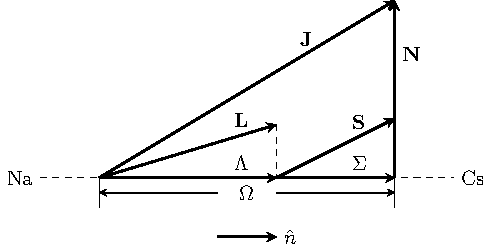
\includegraphics[width=\textwidth]{figures/pa_hunds_case_a.pdf}
  \caption[Hund's case (a)]{
    Angular momentum coupling for \textit{Hund's case (a)}.
    $\mathbf{L}$ and $\mathbf{S}$ are coupled to the internuclear axis $\hat n$
    and the sum of the projections $\Omega=\Lambda+\Sigma$ is then
    added with the orthogonal compoment $\mathbf{N}$ to form $\mathbf{J}$.
    \label{fig:pa-hunds-case-a}}
\end{figure}

This is described by the \textit{Hund's case (a)}.
Molecular states with large binding energies mostly experience interactions
between the atoms at short range where the electric static interaction is very strong.
This couples the the two electron spins into a total electron spin
$\mathbf{S}\equiv\mathbf{S}_1+\mathbf{S}_2$ via a very strong effective interaction
of the form $\mathbf{S}_1\cdot\mathbf{S}_2$ which originates
from the resulting symmetry of the electron orbital wavefunction.
Similar to atoms, the nuclear spin interaction is also very week compared to
other energy scales so we can ignore the hyperfine structure and only need to consider
$\mathbf{J}\equiv\mathbf{L}+\mathbf{S}+\mathbf{N}$.

The strong electrostatic interaction also creates an effective coupling
between the $\mathbf{L}$ and $\mathbf{S}$ with the internuclear axis $\hat{n}$
causing $\mathbf{L}$ and $\mathbf{S}$ to process rapidly around $\hat{n}$.
This creates two new conserved quantity $\Lambda$ and $\Sigma$
as the projection of $\mathbf{L}$ and $\mathbf{S}$
along $\hat{n}$ respectively.
The total angular momentum along $\hat{n}$ is therefore $\Omega\equiv\Lambda+\Sigma$
and it is added to the $\mathbf{N}$ which is orthogonal to $\hat{n}$ to form
the total angular momentum $\mathbf{J}$ (Fig.~\ref{fig:pa-hunds-case-a}).

The angular momenum state of the molecule is therefore fully characterized by
$|L,\Lambda,S,\Omega,J\rangle$. $\Lambda$ can be $0,1,\dots,L$, $\Omega$ ranges from
$\abs{\Lambda-S}$ to $\Lambda+S$ and $J\geqslant\Omega$.
The $L$ quantum number is specified by the electronic state and will be discussed
in section \ref{ch:pa:pes} and the rest of the angular momentum quantum numbers
are represented by the \textit{Hund's case (a)} term symbol,
\[ ^{2S+1}\Lambda_\Omega \]
similar to the atomic term symbol $^{2S+1}L_J$.
Just as the use of capital English letters $S,P,D,\dots$ to represent
$L=0,1,2,\dots$, capital Greek letters $\Sigma,\Pi,\Delta,\dots$ are used
to denote $\Lambda=0,1,2,\dots$ in the term symbol.
An additional symmetry to consider is the reflection about a plane that includes
the internuclear axis.
For $\Lambda>0$ states, the reflection produces a new state at the same energy
creating the so-called $\Lambda$-doubling. For $\Lambda=0$ states, i.e. $\Sigma$ states,
the reflection produces the same state with a phase of $\pm1$.
This phase is also included in the term symbol to fully specify the symmetry of
a $\Sigma$ states as
\[ ^{2S+1}\Sigma_\Omega^{\pm} \]
Note the $\Sigma$ state here should not be confused with the quantum number $\Sigma$.

From the angular momentum relation in Fig.~\ref{fig:pa-hunds-case-a},
we can also determine the energies of different rotational states.
The nuclear rotational energy is given by,
\[
  E_{rot}=B\langle \mathbf{N}^2 \rangle
\]
where $B$ is the rotational constant of the molecule.
For \textit{Hund's case (a)} this is,
\begin{align*}
  E_{rot}=&B\langle \mathbf{J}^2 - \Omega^2 \rangle\\
  =&B\langle \mathbf{J}^2 - \Omega^2 \rangle\\
  =&B\paren{J\paren{J+1}-\Omega^2}
\end{align*}
For the last step, note that $\Omega$ is not an angular momentum vector but a projection.
We can easily see that for a given $\Omega$, we have $J\geqslant\Omega$.
Unlike a rigid rotor where $E_{rot}=BN\paren{N+1}$,
the limit on the $J$ means that the spacing between the rotational levels depend on $\Omega$,
\[2\Omega+2,\ 2\Omega+4,\ 2\Omega+6,\ \dots\]
This allows us to determine the $\Omega$ of the state we are addressing
by measuring the state spacing for the lowest few rotational states.

\subsubsection{Near Threshold Bound States}
\label{pa:structure:near-threshold}

For molecular states with small binding energy, the interaction between the two atoms is
small compared to the internal coupling in the atoms and
the angular momentum coupling is ``atom like''.
In this limit, the total angular momentum $\mathbf{F}_1$ and $\mathbf{F}_2$
for the individual atoms forms $\mathbf{F}_{atom}=\mathbf{F}_1+\mathbf{F}_2$
which is then coupled to the nuclear rotation $\mathbf{N}$
to form $\mathbf{F}=\mathbf{F}_{atom}+\mathbf{N}$.
We will discuss this regime in more detail
when we characterize the weakly bound ground states in chapter \ref{ch:raman-spectroscopy}.

\subsection{Potential Energy Surface}
\label{ch:pa:pes}

Due to the different angular momentum coupling in different regimes,
there is not a consistent way to label the interaction between the two atoms
at both short and long distance.
Nevertheless, by convention, we use the \textit{Hund's case (a)} term symbol
since it more accurately represents the state when the interaction energy dominates.

The Hamiltonian (excluding spin for simplicity\footnote{Electron spin is implicitly included,
  however, via the symmetry of the electronic wavefunction.}) is,
\begin{align*}
  H=&H_e+T_n
\end{align*}
where the electronic term $H_e$ and the nuclear kinetic term $T_n$ are given by
\begin{align*}
  H_e=&-\sum_i\frac{\hbar}{2m_e}\mathbf{\nabla}_i^2+\frac{e^2}{4\pi\varepsilon_0}\paren{\sum_{i>j}\frac{1}{\abs{\mathbf{r}_i-\mathbf{r}_j}}-\sum_{A=\Na,\Cs}\sum_i\frac{Z_{A}}{\abs{\mathbf{r}_i-\mathbf{R}_{A}}}+\frac{Z_{\Na}Z_{\Cs}}{\abs{\mathbf{R}_{\Cs}-\mathbf{R}_{\Na}}}}\numberthis{eq:pa:pes:he}\\
  T_n=&-\sum_{A=\Na,\Cs}\frac{\hbar^2}{2m_{A}}\mathbf{\nabla}_{A}^2
\end{align*}
and the sum is over all the electrons in the molecule.

\subsubsection{Born-Oppenheimer Approximation}

The Hamiltonian is solved using the Born-Oppenheimer (BO) approximation.
Because of the large mass difference between the nuclei and the electrons,
we can assume that the electron motion follows the position of the nuclei
instantaneously so that the motion of the nuclei and the elctrons can be treated separately.
Formally, this mean that the electron wavefunctions is solved using the
electrionic term $H_e$ for a given nuclear position $\mathbf{R}_{\Na}$ and $\mathbf{R}_{\Cs}$.
This results in an effective potential $V_{eff}\paren{\abs{\mathbf{R}_{\Na}-\mathbf{R}_{\Cs}}}$ called
the potential energy surfaces (PES) for each electronic states.
The solutions to the approximate Hamiltonians $T_n+V_{eff}$ provide
the vibrational and rotational states of the molecule.

\subsubsection{Franck-Condon Factor}

In additional to the energy of the molecular bound state,
the solution of the nuclear motion also provides information to the selection rules
and coupling strength of transitions between the states.
For an electronic electric dipole transition between state
$|e_1,v_1,j_1\rangle$ and $|e_2,v_2,j_2\rangle$,
where $e_i$, $v_i$ and $j_i$ denotes electronic, vibrational and angular momentum states,
the Rabi frequency under the BO approximation is,
\begin{align*}
  \Omega=&\langle e_1,v_1,j_1|e\mathbf{r}_e\cdot\mathbf{E}\ue^{\ui\mathbf{k}\cdot\mathbf{r}}|e_2,v_2,j_2\rangle\\
  =&\langle e_1(\mathbf{r})|e\mathbf{r}_e\cdot\mathbf{E}|e_2(\mathbf{r})\rangle\langle v_1,j_1|\ue^{\ui\mathbf{k}\cdot\mathbf{r}}|v_2,j_2\rangle
\end{align*}
where $\mathbf{r}$ and $\mathbf{r}_e$ are the molecule and electron coordinates.
For most of the transitions, we can treat the nuclear coordinate dependent transition dipole
moment $\mathbf{D}\paren{\mathbf{r}}\equiv\langle e_1(\mathbf{r})|e\mathbf{r}_e|e_2(\mathbf{r})\rangle$ as a constant $\mathbf{D}$.
Since the size of the molecular wavefunction is also usually much smaller than
the wavelength of the transition, we can also assume $\ue^{\ui\mathbf{k}\cdot\mathbf{r}}\approx 1$,
we have,
\begin{align*}
  \Omega=&\mathbf{D}\cdot\mathbf{E}\langle j_1|j_2\rangle\langle v_1|v_2\rangle
\end{align*}
The term $\langle j_1|j_2\rangle$ determines the angular momentum selection rule which is
$\Delta\Lambda=0,\pm1$, $\Delta S=\Delta\Sigma=0$, $\Delta\Omega=0,\pm1$ and $\Delta J=0,\pm1$
for \textit{Hund's case (a)}\cite{straughan_spectroscopy_1976}.
The term $\langle v_1|v_2\rangle$ gives the coupling strength between vibrational states
\footnote{Note that $\langle v_1|v_2\rangle$ does not simplify to orthogonality relation
  when $e_1\neq e_2$ since the vibrational wavefunctions belongs to different PES.}.
This is called the Franck-Condon principle and the square of the wavefunction overlap
is defined as the Franck-Condon factor (FCF),
\begin{align*}
  \mathrm{FCF}\equiv&\abs{\langle v_1|v_2\rangle}^2
\end{align*}
For incoherent transition, the transition rate is proportional to $\Omega^2\propto\mathrm{FCF}$.

\subsubsection{Energy Level of $\mathrm{NaCs}$}

\begin{figure}
  \centering
  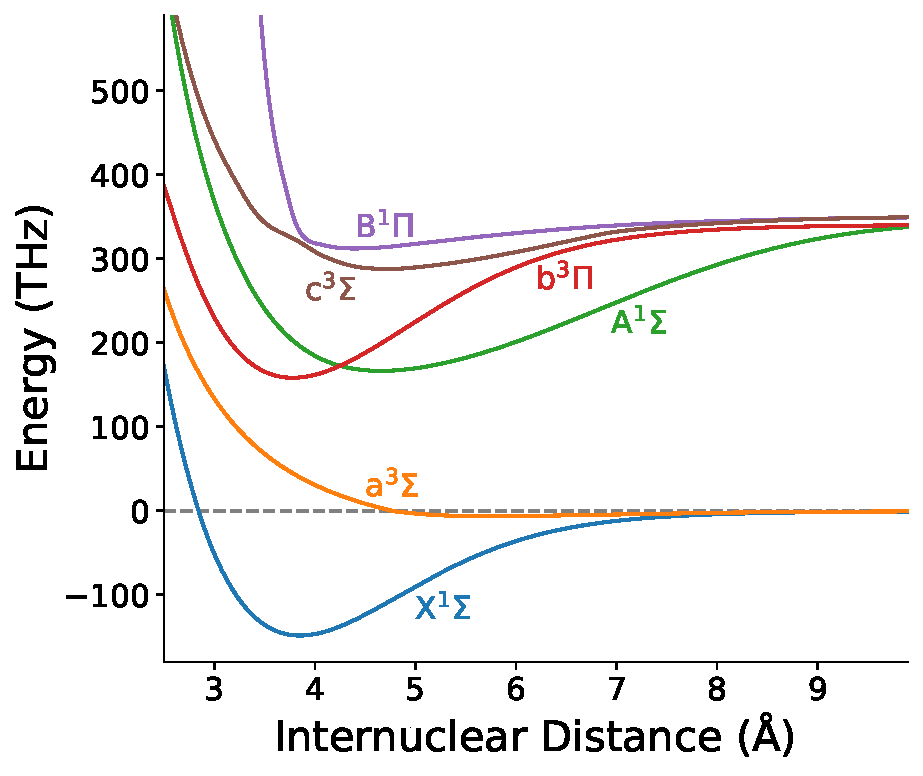
\includegraphics[width=0.9\textwidth]{figures/pa_pes.pdf}
  \caption[NaCs potential energy surfaces]{
    Potential energy surfaces of NaCs with \textit{Hund's case (a)} labels.
    Due to spin-orbit coupling, the potentials are not independent of each other.
    The real energy eigenstates of the molecule may be a superposition of multiple
    electronic and spin states.
    \label{fig:pa-pes}}
\end{figure}

Fig.~\ref{fig:pa-pes} shows the relevant PESs for $\mathrm{NaCs}$.
Although the spin-less electronic Hamiltonian \ref{eq:pa:pes:he} makes it easier
to understand the molecule structure and provides good approximations for the
transition dipoment and FCF, the absense of spin and the difficulty in exactly solving
a multi-electron system makes it unsuitable to calculate energy levels
for spectroscopy purpose.
Because of this, prediction of the molecular states energies are calculated using
PESs fitted to experimental data\cite{docenko_coupling_2006,zaharova_solution_2009,grochola_spin-forbidden_2011,grochola_investigation_2010}.

\section{Photoassociation Spectroscopy}
\label{pa:pa}

\subsection{Beampath}
\label{pa:beampath}

\begin{figure}
  \centering
  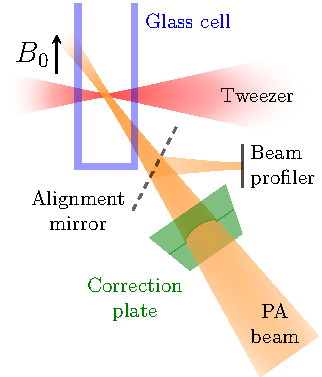
\includegraphics[width=0.7\textwidth]{figures/pa_beampath.pdf}
  \caption[PA beampath]{
    PA beampath including the relative geometry with the magnetic field
    the glass vacuum cell and the tweezer.
    In order to compensate for the astigmatism from pass through the glass cell window
    at an angle, we added an correction glass plate into the PA beam path.
    The correction plate has the same thickness and angle of incident with the glass cell window
    but is angled vertically instead of horizontally.
    The alignment mirro and the beam profiler can also be added to the beam path
    in order to measure the chromatic error during alignment.
    \label{fig:pa-beampath}}
\end{figure}

The excited molecular state we would like to address has a bond length of $3-8\AA$.
The initial atomic state, however, has an average inter-nuclear distance of $\approx1000\AA$.
This size mismatch between the initial and final state wavefunctions
means the transition typically have a very small FCF ($10^{-10}-10^{-8}$).
Because of this, we focus our PA beam onto the tweezer with a beam waist between
$10\mathrm{\mu m}$ and $30\mathrm{\mu m}$ (Fig.~\ref{fig:pa-beampath}) in order to
increase the laser intensity and improve the signal contrast.
The tight focus also increase the astigmatism when passing through
the glass cell window at an angle which limits the minimum focus size we can achieve.
Therefore, we added a correction glass plate to fix the astigmatism
in order to minimize the focus size and maximize the beam intensity.

\begin{figure}
  \centering
  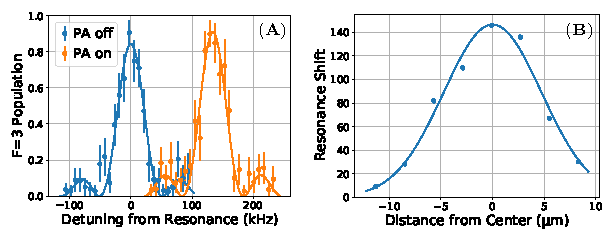
\includegraphics[width=\textwidth]{figures/pa_vectorshift.pdf}
  \caption[PA beam alignment]{
    Measurement of Cs vector light shift from the PA beam for final alignment.
    (A) The effective magnetic field from the circularly polarized PA beam
    causes a shift on the Raman resonance between the $|4,4\rangle$ and $|3,3\rangle$ states.
    (B) Vector light shift as a function of PA beam position
    used to determine the beam center.
    The $1/\ue$ diameter of the beam is measured to be $13.40(72) \mathrm{\mu m}$.
    \label{fig:pa-alignment}}
\end{figure}

In order to align the PA beam to the tweezer, we use the following alignment procedure,
\begin{enumerate}
\item Light resonant with the Cs atomic transition is sent into the PA beam path.
  This allows us to do the alignment using the procedure we used to align the
  atomic Raman sideband cooling beams as described in section \ref{ch:rsc:alignment}.
  However, unlike the alignment for the atomic Raman beams,
  due to the larger frequency difference between the PA transition and the Cs atomic
  transition as well as the smaller beamsize,
  we cannot use the alignment result from this step directly for the PA beam
  due to the chromatic aberration from the optics in the PA beam path.
\item In order to translate the alignment result from resonance Cs light to that of the PA light,
  we insert a mirror to reflect the PA beam after the last optics in the beam path
  and place a beam profiler at the equivalent location of the tweezer
  (Fig.~\ref{fig:pa-beampath}).
  This allow us to directly measure location of the focal point for the two wavelengths
  and correct for the chromatic aberration by shifting the focus from the PA light
  to the original focus position from the resonance Cs light.
\item As the final alignment step and to correct for the chromatic aberration of the
  glass window that was not corrected for in the last step,
  we align the PA beam to the atom using signal directly from the atom.
  Due to the large detuning, the scattering rate from the PA beams
  is too low to be used for alignment.
  However, when the PA beam is set to circular polarization, it creates an effective
  magnetic field parallel to the beam propagation direction
  of the form\cite{thompson_coherence_2013},
  \[ B_{eff}=-U_0\frac{\delta_2-\delta_1}{\delta_2+2\delta_1}\mathbf{C} \]
  where $U_0$ is the scalar light shift, $\delta_1$ and $\delta_2$ are the detuning from the
  $\mathrm{D}_1$ and $\mathrm{D}_2$ line respectively,
  $\mathbf{\varepsilon}$ is the polarization vector and
  $\mathbf{C}\equiv\Im\paren{\mathbf{\varepsilon}\times\mathbf{\varepsilon}^*}$
  qualifies the ellipticity of the polarization with
  $\abs{C}=1$ for pure circular polarization and $\abs{C}=0$ for linear polarization.
  This effective magnetic field causes a relative shift between the $|4,4\rangle$
  and the $|3,3\rangle$ states which can be measured using a Raman transition
  (Fig.~\ref{fig:pa-alignment}A).
  By measuring the shift as a function of the beam position,
  we can determine the size and the center of the PA beam and align the beam to the atom
  (Fig.~\ref{fig:pa-alignment}B).
\end{enumerate}

\subsection{Experiment Sequence and Resonance Frequencies}
\label{pa:sequence-res}

For the PA spectroscopy, we mainly focus on states with large binding energies
which are expected to be good candidates as the intermediate state
for Raman transfer\textsuperscript{(\ref{ch:raman-transfer:raman-model})}.
In particular, we scanned the PA light frequency around the $v'=0$ and $v'=12-14$
vibrational states in the $c^3\Sigma$ potential.

In order to observe PA, we first prepare both the Na and Cs atoms in the motional ground states
in the same tweezer\cite{liu_building_2018}.
We then turn on the PA beam for a set time
followed by separating the atoms into their respective tweezers and image the atoms.
When we hit a PA resonance, the excited molecular state will typically decay down
to either a molecular ground state,
which will remain in at most one of the tweezers after the separation,
or an atomic state with high relative motional energy and escape the trap.
In either case, this leads to at least one empty tweezer after the separation.
By measuring the probability of having both the Na and Cs atoms after the PA pulse
conditioned on both atoms being initially loaded,
we can capture the probability of PA event and locate the resonances.

\todo{
  Theory prediction and results
}

The initial atomic state we used is $|\mathrm{Na(2, 2),Cs(4, 4)}\rangle$
which has $L=0$ and $S=1$.
For atoms in the motional ground state we also have $N=0$ and therefore $J=1$
which should be coupled to $J=0,1,2$ excited states from the $\Delta J=0,\pm1$ selection rule.
However, since the cooling is not perfect,
we expect some atoms initially in the $N=1$ state which can allow a weaker
transition to the $J=3$ states.

\todo{
  Spin assignment
}

\todo{
  Theory prediction for v'=0
  (NaCs 2017-2018 > NaCs 2018 > Raman transfer plan to v=-1 > c3Sigma v=0 frequency prediction)
  J states? (NaCs 2017-2018 > NaCs 2018 > c3Sigma v=0 search > Scan 4/16-4/18)
}

\subsection{Linewidth}
\label{pa:linewidth}

In additional to the energy, another property of the excited state
that is important for driving a two-photon transition using the state is the linewidth.
This determines the scattering or decoherence rate of
the two-photon transition which then determines
the transfer efficiency\textsuperscript{(\ref{ch:raman-transfer})}.
The linewidth, or decay rate, due to electric dipole transitions is,
\begin{align*}
  \Gamma=&\sum_{i}\frac{\omega_i^3d_i^2\mathrm{FCF}_i}{3\pi\varepsilon_0\hbar c^3}
\end{align*}\todo{check and \cite{}}
where $\omega_i$ is the decay frequency, $d_i$ is the transition dipole moment,
and the sum is over all the decay channels.
Since the size of the excited state electron wavefunction is similar to that of the atom
the molecule has a similar transition dipole moment as the corresponding atomic transition
$d_i\approx d_\Cs$. Moreover, since $\sum_i\mathrm{FCF}_i=1$ and $\omega_i\approx\omega_\Cs$
we have
\begin{align*}
  \Gamma\approx&\frac{\omega_\Cs^3d_\Cs^2}{3\pi\varepsilon_0\hbar c^3}\\
  =&\Gamma_\Cs\approx2\pi\cdot5\mathrm{MHz}
\end{align*}\todo{check and \cite{}}
Since the PA laser is locked using a wavemeter with a precision
$\approx20\mathrm{MHz}$, we expect the PA linewidth we measured to be limited
by our frequency resolution.

This is, however, not what is observed in the experiment.
Fig~.\todo{\ref{}} shows the narrowest spectrum of the $v=\todo{number}$ PA line
we measured when the tweezer frequency is set to $...\todo{}$
with $...\todo{} \mathrm{mW}$ of power. The linewidth is determined to be $... \mathrm{MHz}$
which is much greater than the theory prediction.

Furthermore, the observed linewidth appears to be dependent on the tweezer power.
The same PA line measured with $...\todo{} \mathrm{mW}$ tweezer power
is shown in Fig~.\todo{\ref{}} with a significantly narrower linewidth
of $... \mathrm{MHz}$.
Fig~.\todo{\ref{}} shows that the linewidth is proportional to the tweezer power
which suggests that the linewidth may be broadened by a two photon process.

We initially suspected that the source of this broadening is due to the tweezer light
coupling the excited molecular state to another state at a higher energy. \todo{figure}
If this is the case, we would expect the broadening to be a function of
the sum of the tweezer and PA light frequency depending on the detuning from the nearest
two photon excited state.
However, the broadening does not change significantly when the tweezer frequency
is changed by $\approx10\mathrm{GHz}$ and
is also observed for other excited states including \todo{$v=...$}
which has very different resonance frequency.
It is therefore unlikely that this is the broadening mechanism we observe.
Instead, we believe the effect is caused by a $\Lambda$ type two photon process
coupling the excited state to the atomic ground states.
In the following section, I will provide an estimation for such a broadening process.

\subsubsection{Two Photon Coupling to the Atomic Motional Continuum}
The broadening of the PA line requires coupling the excited state to a continuum of states.
For the ground atomic state, since the state is stable with repect to radiative decay,
this continuum cannot be the photon continuum.
Instead, the excited state is coupled to the relative motional continuum of the atoms.
Physically, this corresponds to a photodissociation process
where the atoms flies away with high kinetic energies corresponding
to the detuning of the tweezer.\todo{figure}

The photodissociation rate is determined by the Fermi's golden rule,
\[
  \Gamma=2\pi\Omega_{if}^2\ \rho_f
\]
where $\Omega_{if}$ is the matrix element between the initial and final state
and $\rho_f$ is the density of state near the final state.
We calculate this by first discretizing the continuum and the rate becomes
\[
  \Gamma=2\pi\frac{{\Omega'_{if}}^2}{\delta}
\]
where $\Omega'_{if}$ is the Rabi frequency between the initial and final state
and $\delta$ is the spacing between the discretized final states.

The Rabi frequency $\Omega'_{if}$ is proportional to the square root of FCF,
which we calculate for the atomic ground motional states by exactly diagonalization
of the atomic wavefunction.
However, due to the high energy $>10\mathrm{GHz}$ of the final state,
calculating FCF for the target state using this method requires an unrealiztic number of
states to be included.
Instead, we approximate it using the results for the atomic ground state
by assuming the FCF to be proportional to the probability density of non-interacting
atomic wavefunction at zero relative distance so that,
\[
  \Omega'_{if}=\Omega_0\frac{\psi_f\paren{r_{rel}=0}}{\psi_0\paren{r_{rel}=0}}
\]
where $\Omega_0$ is the Rabi frequency between the excited state and
the atomic motional ground state and $\psi_f$ and $\psi_0$ are the
wavefunctions of the final and ground motional atomic state without the molecular potential.
This approximation is justifed because,
\begin{enumerate}
\item The molecular potential is short ranged and the excited molecular state is small.
\item Only the final atomic wavefunction within the molecular potential contributes to the FCF.
  For relatively low motional energy
  this wavefunction is proportional to the value of the wavefunction at
  the edge of the molecular potential which is well approximated by
  the atomic wavefunction without the molecular potential.
  \todo{figure}
\end{enumerate}
This approximation remains valid until the de Broglie wavelength for the atomic state
is comparable to the size of the molecular potential which corresponds to
a motional energy of $\approx40\mathrm{GHz}$
and the result can still be used as order of magnitude estimation for higher motional energies.

For atomic motional ground state, we have,
\begin{align*}
  \psi_0\paren{r_{rel}=0}=&\prod_{i=1}^{3}\paren{\frac{\mu\omega_i}{\pi}}^{1/4}\\
  =&\paren{\frac{\mu^3\omega_1\omega_2\omega_3}{\pi^3}}^{1/4}
\end{align*}
where $\mu$ is the reduced mass $\mu\equiv m_\Na m_\Cs/\paren{m_\Na+m_\Cs}$,
and $\omega_i$'s are the relative trapping frequencies along the three trap axis.
We discretize the continuum state by adding an infinitely deep spherical potential well
of radius $R$ around the center. The radial wavefunctions of the eigenstates
within the well with quantum number $n=1,2,\dots$ is,
\begin{align*}
  \psi_n=&\frac{1}{\sqrt{4\pi}r_{rel}}\sqrt{\frac{2}{R}}\sin\paren{\frac{\pi nr_{rel}}{R}}
\end{align*}
and the corresponding energy,
\begin{align*}
  E_n=&\frac{\pi^2n^2}{2\mu R^2}
\end{align*}
The energy gap between neighboring states is
\begin{align*}
  \delta_n\approx&\frac{\pi^2n}{\mu R^2}
\end{align*}
and the wavefunction value at $r_{rel}=0$ is,
\begin{align*}
  \psi_n\paren{r_{rel}=0}=&\sqrt{\frac{1}{2\pi R}}\left.\frac{\ud}{\ud r_{rel}}\sin\paren{\frac{\pi nr_{rel}}{R}}\right|_{r_{rel}=0}\\
  =&\frac{\pi n}{\sqrt{2\pi R}R}
\end{align*}
Substituting into $\Gamma$ and taking the limit of $R\rightarrow\infty$ we have
\begin{align*}
  \Gamma=&2\pi\frac{\Omega_0^2}{\delta}\frac{\psi_f^2\paren{r_{rel}=0}}{\psi_0^2\paren{r_{rel}=0}}\\
  =&2\pi\Omega_0^2\frac{\mu R^2}{\pi^2n}\frac{\pi^2 n^2}{2\pi R^3}\sqrt{\frac{\pi^3}{\mu^3\omega_1\omega_2\omega_3}}\\
  =&\Omega_0^2\frac{n}{R}\sqrt{\frac{\pi^3}{\mu\omega_1\omega_2\omega_3}}\\
  =&\Omega_0^2\sqrt{\frac{2\pi E}{\omega_1\omega_2\omega_3}}
\end{align*}
For the condition in Fig.~\todo{\ref{}} we have $\Omega_0=2\pi\cdot\todo{number}...$,
$E=2\pi\cdot\todo{number}...$ and $\omega_{1,2,3}=2\pi\cdot\todo{number}...$
which predict a broadened linewidth of $\Gamma=2\pi\cdot\todo{number}...$.
This prediction is only an estimate due to due to the breakdown of the approximation
we used and is in fact broader than the observed value.
Nevertheless, it confirms that this broadening mechanism can explain the observed linewidth.

\todo{Acknowedge Olivier}
\todo{
  Implication on two-photon transfer
}
